\documentclass[tikz]{standalone}
\usepackage{pgfplots}
\usepackage{amsmath}
\pgfplotsset{compat=1.18}

\begin{document}
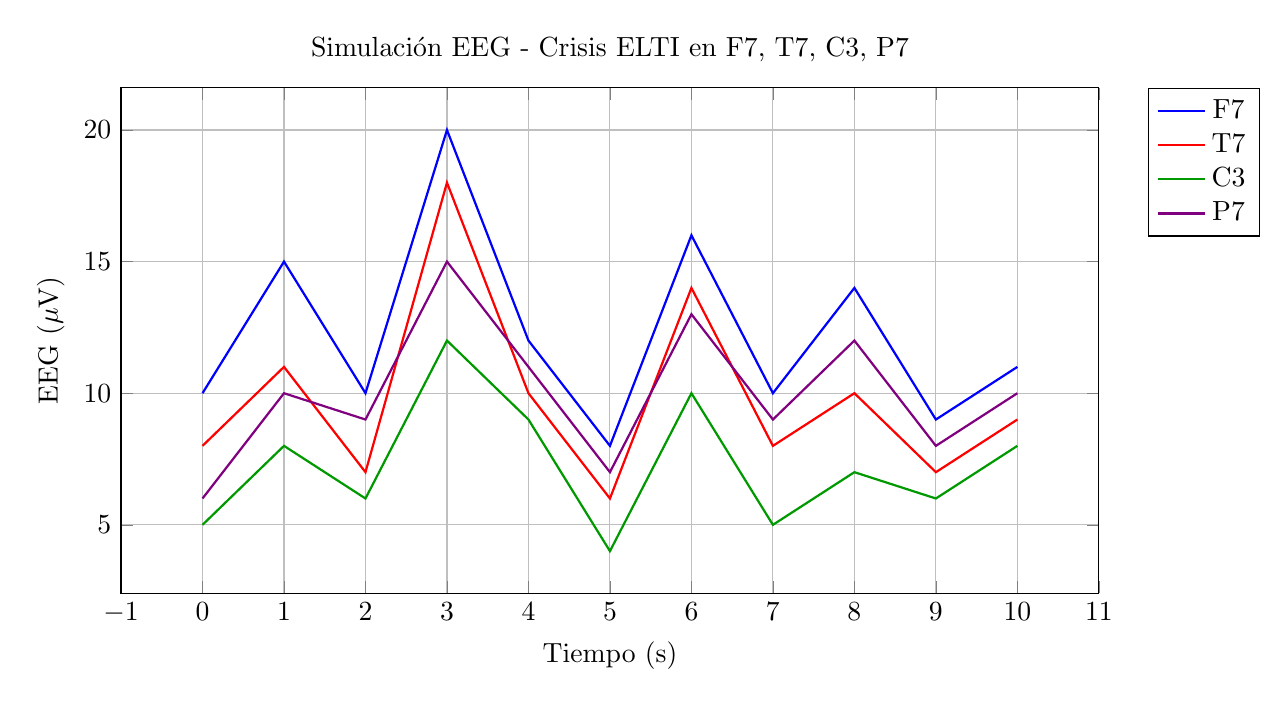
\begin{tikzpicture}
\begin{axis}[
    width=14cm,
    height=8cm,
    xlabel={Tiempo (s)},
    ylabel={EEG ($\mu$V)},
    title={Simulación EEG - Crisis ELTI en F7, T7, C3, P7},
    legend style={at={(1.05,1)}, anchor=north west},
    grid=both
]
\addplot+[no marks, thick, blue] table {
0 10
1 15
2 10
3 20
4 12
5 8
6 16
7 10
8 14
9 9
10 11
};
\addlegendentry{F7}

\addplot+[no marks, thick, red] table {
0 8
1 11
2 7
3 18
4 10
5 6
6 14
7 8
8 10
9 7
10 9
};
\addlegendentry{T7}

\addplot+[no marks, thick, green!60!black] table {
0 5
1 8
2 6
3 12
4 9
5 4
6 10
7 5
8 7
9 6
10 8
};
\addlegendentry{C3}

\addplot+[no marks, thick, violet] table {
0 6
1 10
2 9
3 15
4 11
5 7
6 13
7 9
8 12
9 8
10 10
};
\addlegendentry{P7}

\end{axis}
\end{tikzpicture}
\end{document}
